\documentclass[usenames, xcolor=dvipsnames]{beamer}
%% \documentclass[professionalfonts, xcolor=table, handout]{beamer}
%% \usepackage{pgfpages}
%% \pgfpagesuselayout{4 on 1}[a4paper,border shrink=5mm, landscape]
\usepackage{fontspec}
\usepackage{amsmath,amssymb}
\usepackage{pifont}% http://ctan.org/pkg/pifont
\usepackage{tikz}
\usetikzlibrary{positioning, matrix, arrows.meta, shapes.geometric, calc,
  decorations.pathmorphing, decorations.pathreplacing, fit, shapes.multipart}
\usepackage{mathabx}
\usepackage{mathtools}
\usepackage{mathpartir}
\usepackage{fancyvrb}
\usepackage{stmaryrd}
\usepackage[absolute,overlay]{textpos}
\definecolor{lightg}{RGB}{217,232,225}
\definecolor{darkg}{RGB}{6,81,42}
\definecolor{myred}{rgb}{0.89, 0.45, 0.36}
\colorlet{mypink}{myred!50!white}
\colorlet{mymaroon}{red!70!black}

\defaultfontfeatures{Mapping=tex-text,Scale=MatchLowercase}
% \setmainfont{Libertinus Serif}
% \setsansfont{Libertinus Sans}
% \setmonofont{Menlo Regular}
\usetheme{Madrid}
\useoutertheme{infolines} % Alternatively: miniframes, infolines, split
\useinnertheme{circles}

% \setbeamertemplate{enumerate item}[default]
\usecolortheme[named=myred]{structure}
% \usecolortheme{spruce}
\usefonttheme{serif}
\setbeamerfont*{frametitle}{series=\bfseries}
\setbeamercolor{alerted text}{fg=mymaroon}
\setbeamertemplate{navigation symbols}{}
\setbeamercolor{emphC}{fg=myred}
% \setbeamercolor{block title}{bg = darkg, fg=white!80}
% \setbeamercolor{block body}{bg = lightg, fg=black}
\setbeamercolor{itemize item}{fg=black}
\setbeamercolor{description item}{fg=myred}

\newcommand{\scon}{\mathbin{\ast}}
\newcommand{\ocon}{%
  \mathbin{\mbox{$\mathrlap{\cup}\hspace*{.15em}
      \raisebox{.01em}[0ex][0ex]{$\scon$}$\hspace*{.07em}}}}
\newcommand{\medocon}{
  \raisebox{-0.3ex}{\resizebox{0.63em}{!}{$\scon$}} \hspace{-2.4ex} \bigcup}
\newcommand{\wand}{%
 \mathrel{\mbox{$\hspace*{-0.03em}\mathord{-}\hspace*{-0.66em}
  \mathord{-}\hspace*{-0.36em}\mathord{\scon}$\hspace*{-0.005em}}}}
\newcommand{\defeq}{\mathbin{\overset{\mathrm{def}}{=}}}
\newcommand{\emphd}[1]{{\bfseries #1}}
\newcommand{\emphr}[2]{\alert<#1>{#2}}
\newcommand{\bracket}[1]{[#1]}
\newcommand{\hide}[1]{}
\newcommand{\braces}[1]{\left\{\begin{array}{l@{}} #1 \end{array}\right\}}

\makeatletter\let\frametextheight\beamer@frametextheight\makeatother
\newcommand\credit[1]{%
  \begin{textblock*}{\paperwidth}(0pt,\textheight)
    \raggedleft #1\hspace{.5em}
\end{textblock*}}
\newcommand{\pguards}[1]{\llbracket #1 \rrbracket}
\newcommand{\xmark}{\ding{55}}%
\newcommand{\cmark}{\ding{51}}%
\newcommand{\m}[1]{\ensuremath{\mathit{#1}}} % math font
\newcommand{\sz}{\texttt{SIZE}}
\newcommand{\ifty}{\texttt{INF}}
\newcommand{\p}[1]{\ensuremath{\mathsf{#1}}} % predicate font
\newcommand{\bi}{\Leftrightarrow} % equivalence of expressions


\title[Verified GC for Gallina]{A Verified Garbage Collector for Gallina}
\author[Wang, Mohan, Cao, Hobor]{\hspace{-0.5em}Shengyi Wang$^\dagger$, 
\underline{Anshuman Mohan}$^\dagger$, Qinxiang Cao$^\ddagger$, Aquinas Hobor$^\dagger$}
\institute[]{$\includegraphics[height=0.12\textwidth]{NUS_logo_full-horizontal.jpg}
  ~\raisebox{2em}{$(\dagger)$}$
  $\qquad \qquad \qquad$ $\includegraphics[height=0.12\textwidth]{sjtubannerblue.png}~
  ~\raisebox{2em}{$(\ddagger)$}$ \hspace*{-1.25em}}
  \date[APLAS NIER 2019]{APLAS NIER \\ \today}

\begin{document}
\begin{frame}[plain]
  \titlepage
\end{frame}

\section{Introduction}

\begin{frame}{Broad Problem}
Verify \alert{graph-manipulating} programs
\\ \hspace{1em}written in \alert{executable C}
\\ \hspace{2em}with \alert{machine-checked} correctness proofs
\bigskip
\uncover<2->{\flushright{Hard, but ubiquitous in critical areas}}
\end{frame}

\begin{frame}{Broad Solution}
\includegraphics[scale=0.09]{vst_logo}
\hspace{2em} \includegraphics[scale=0.12]{compcert_logo}
\hspace{2em} \includegraphics[scale=0.2]{paper_screen}

\bigskip
VST + CompCert + 25000 \textsc{loc} library

\pause
\bigskip
Powerful enough to verify \alert{executable code}
\\\hspace{1em}against \alert{realistic specifications}
\\\hspace{2em}expressed with \alert{mathematical graphs}

\pause 
\bigskip
\flushright [{\footnotesize Wang \emph{et. al.}}, \textsc{pacmpl oopsla} {\footnotesize 2019}]
\end{frame}

\begin{frame}{This Talk}
\includegraphics[scale=0.02]{certicoq_logo} 
\hspace{2em} \includegraphics[scale=0.12]{compcert_logo}

\bigskip
Gallina \alert<2->{$\leadsto$} CompCert C $\leadsto$ Assembly

\bigskip \pause
Gallina assumes \alert{infinite} memory
\\\hspace{1em} but CompCert C has a \alert{finite} heap

\bigskip
\pause Solution: garbage collect the CompCert C code

\pause
\flushright{\alert{New problem: verify the garbage collector}}
\end{frame}

\section{Specification}

\begin{frame}{Our Garbage Collector}
\uncover<1->{GC has jurisdiction over the heap}
\uncover<3->{\\\hspace{1em} Mutator $\texttt{alloc}$s in special subheap}
\uncover<4->{\\\hspace{2em} If subheap is full} 
\uncover<5->{\alert{call GC}}
\uncover<6->{and try again}

\bigskip

\begin{center}
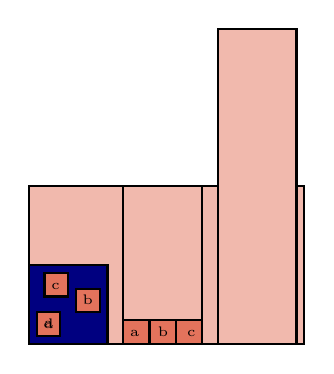
\begin{tikzpicture}
\uncover<1>{\draw [fill=mypink, thick] 
  (0,0) -- (3.5,0) -- (3.5,2) -- (0,2) -- cycle;}
\uncover<2->{\draw [fill=mypink, thick] 
  (0,0) -- (1,0) -- (1,1) -- (0,1) -- cycle;
            \draw [fill=mypink, thick] 
  (1.2,0) -- (2.2,0) -- (2.2,2) -- (1.2,2) -- cycle;
            \draw [fill=mypink, thick] 
  (2.4,0) -- (3.4,0) -- (3.4,4) -- (2.4,4) -- cycle;}
\uncover<3,6>{\draw [fill=myred, thick]
  (0.1,0.1) -- (0.4,0.1) -- (0.4,0.4) -- (0.1,0.4) -- cycle;}
\uncover<4>{\draw [fill=NavyBlue, thick]
  (0,0) -- (1,0) -- (1,1) -- (0,1) -- cycle;
            \draw [fill=myred, thick]
  (0.1,0.1) -- (0.4,0.1) -- (0.4,0.4) -- (0.1,0.4) -- cycle;
            \draw [fill=myred, thick]
  (0.6,0.4) -- (0.9,0.4) -- (0.9,0.7) -- (0.6,0.7) -- cycle;
            \draw [fill=myred, thick]
  (0.2,0.6) -- (0.5,0.6) -- (0.5,0.9) -- (0.2,0.9) -- cycle;
  }
\uncover<5->{\draw [fill=myred, thick]
  (1.2,0) -- (2.2,0) -- (2.2,0.3) -- (1.2,0.3) -- cycle;
  \draw[thick] (1.533,0) -- (1.533,0.3);
  \draw[thick] (1.866,0) -- (1.866,0.3);
  }

\uncover<3-4>{\node at (0.25,0.25){\tiny a};}
\uncover<4>{\node at (0.75,0.56){\tiny b};
            \node at (0.34,0.73){\tiny c};
}
\uncover<5->{\node at (1.7,0.15){{\tiny a} \hspace{0.01em} {\tiny b} \hspace{0.01em} {\tiny c}};}
\uncover<6>{\node at (0.25,0.25){\tiny d};}


\end{tikzpicture}
\end{center}
\end{frame}

\section{Our Garbage Collector}

\begin{frame}{Our Garbage Collector}
  \begin{itemize}
  \item 12 generations, doubling in size
  \item Functional mutator: no back pointers
  \pause
  \item Cheney's mark-and-copy collects gen to next
  \item Potentially triggers cascade of pairwise collections
  \pause
  \item Three key functions: 
  \\\hspace{1em}\texttt{forward} copies individual objects
  \\\hspace{1em}\texttt{do\_scan} repairs copied objects
  \\\hspace{1em}\texttt{forward\_roots} kick-starts the collection
  \end{itemize}
\end{frame}

\begin{frame}{Intuitive Specification}
\emph{Primum non nocere}: first, do no harm

\bigskip

\begin{center}
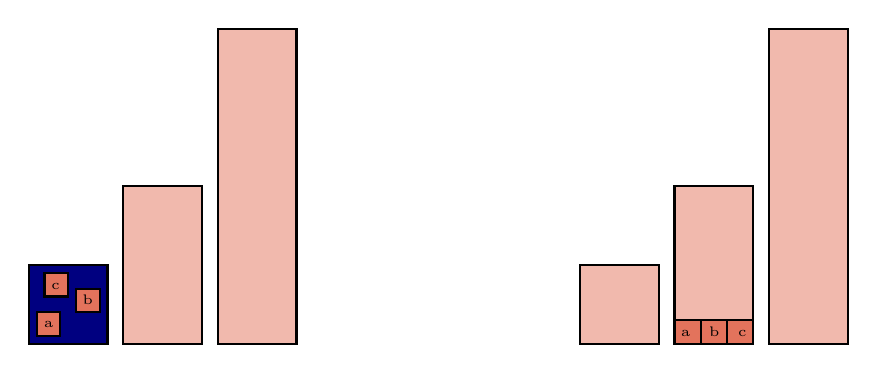
\begin{tikzpicture}
\uncover<1->{
            \draw [fill=NavyBlue, thick]
  (0,0) -- (1,0) -- (1,1) -- (0,1) -- cycle;
            \draw [fill=myred, thick]
  (0.1,0.1) -- (0.4,0.1) -- (0.4,0.4) -- (0.1,0.4) -- cycle;
            \draw [fill=myred, thick]
  (0.6,0.4) -- (0.9,0.4) -- (0.9,0.7) -- (0.6,0.7) -- cycle;
            \draw [fill=myred, thick]
  (0.2,0.6) -- (0.5,0.6) -- (0.5,0.9) -- (0.2,0.9) -- cycle;
            \draw [fill=mypink, thick ] 
  (1.2,0) -- (2.2,0) -- (2.2,2) -- (1.2,2) -- cycle;
            \draw [fill=mypink, thick ] 
  (2.4,0) -- (3.4,0) -- (3.4,4) -- (2.4,4) -- cycle;}

\node at (0.25,0.25){\tiny a};
\node at (0.75,0.56){\tiny b};
\node at (0.34,0.73){\tiny c};

\tikzset{shift={(7,0)}}
  \uncover<2->{
            \draw [fill=mypink, thick ]
  (0,0) -- (1,0) -- (1,1) -- (0,1) -- cycle;
            \draw [fill=mypink, thick ] 
  (1.2,0) -- (2.2,0) -- (2.2,2) -- (1.2,2) -- cycle;
            \draw [fill=mypink, thick ] 
  (2.4,0) -- (3.4,0) -- (3.4,4) -- (2.4,4) -- cycle;
  \draw [fill=myred, thick]
  (1.2,0) -- (2.2,0) -- (2.2,0.3) -- (1.2,0.3) -- cycle;
  \draw[thick] (1.533,0) -- (1.533,0.3);
  \draw[thick] (1.866,0) -- (1.866,0.3);
  \node at (1.7,0.15){{\tiny a} \hspace{0.01em} {\tiny b} \hspace{0.01em} {\tiny c}};}
  \end{tikzpicture}
\end{center}

\uncover<3>{\vspace{-6em}\hspace{5.8cm}\Huge $\cong$}
\end{frame}


\newcommand{\ws}[1]{\color{white}{\tiny #1}}

\begin{frame}[fragile]{Overview of Operations}
\begin{columns}[T] % align columns
\begin{column}{.4\textwidth}

\uncover<1-8>{Nursery cannot fit \texttt{alloc}}

  \hspace{1em}\uncover<2-8>{\texttt{do\_gen}}
\\\hspace{2em}\uncover<3-8>{\texttt{forward\_roots}}
\\\hspace{3em}\uncover<4-8>{\texttt{forward}}
\\\hspace{2em}\uncover<5-8>{\texttt{do\_scan}}
\\\hspace{3em}\uncover<6-8>{\texttt{forward}}
\\\hspace{2em}\uncover<7-8>{\texttt{reset\_gen}}

\vspace{-8.7em}
\uncover<9->{Non-Concerns}
\\\hspace{1em}\uncover<10->{more garbage}
\\\hspace{1em}\uncover<11->{backward pointers}

\bigskip

\uncover<12->{Sources of Complexity}
\\\hspace{1em}\uncover<13->{variable-length objects}
\\\hspace{1em}\uncover<14->{disambiguate int/ptr}
\\\hspace{1em}\uncover<15->{determine \texttt{v}'s gen}
\\\hspace{1em}\uncover<16->{determine gen size}
\\\hspace{1em}\uncover<17->{\color{OliveGreen}what if \texttt{malloc} fails?}


\end{column}%
\hfill%
\begin{column}{.6\textwidth}
  \begin{center}
  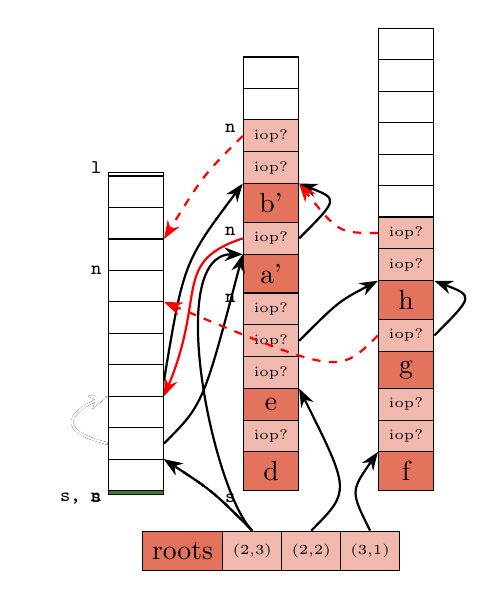
\begin{tikzpicture}[heap/.style={rectangle split, rectangle split parts=#1, draw,
        minimum width=20pt}, node distance=1cm, ->/.style={-Stealth, thick}]
    \node<1-3> [heap=10, rectangle split part fill={white, white, white, mypink, myred, mypink, mypink, myred, mypink, myred}]
    (gen 0) {\nodepart{ten}\ws{a}
            \nodepart{eight}\ws{b}
            \nodepart{five}\ws{c}};
    \node<4,5> [heap=10, rectangle split part fill={white, white, white, mypink, myred, mypink, mypink, myred, mypink, OliveGreen}]
    (gen 0) {\nodepart{ten}\ws{a}
            \nodepart{eight}\ws{b}
            \nodepart{five}\ws{c}};
    \node<6> [heap=10, rectangle split part fill={white, white, white, mypink, myred, mypink, mypink, OliveGreen, mypink, OliveGreen}]
    (gen 0) {\nodepart{ten}\ws{a}
            \nodepart{eight}\ws{b}
            \nodepart{five}\ws{c}};
    \node<7> [heap=10, rectangle split part fill={white, white, white, mypink, NavyBlue, mypink, mypink, OliveGreen, mypink, OliveGreen}]
    (gen 0) {\nodepart{ten}\ws{a}
            \nodepart{eight}\ws{b}
            \nodepart{five}\ws{c}};
    \node<8-> [heap=10, rectangle split part fill={white}] (gen 0) {};

    \node<1-3>[heap=13, right = of gen 0.south east, anchor=south west,
      rectangle split part fill={white, white, white, white, white, white, white, mypink, mypink, mypink, myred, mypink, myred}]
        (gen 1) {\nodepart{thirteen}\ws{d}
                 \nodepart{eleven}\ws{e}};
    \node<4,5>[heap=13, right = of gen 0.south east, anchor=south west,
      rectangle split part fill={white, white, white, white, white, mypink, myred, mypink, mypink, mypink, myred, mypink, myred}]
        (gen 1) {\nodepart{thirteen}\ws{d}
                 \nodepart{eleven}\ws{e}
                 \nodepart{seven}\ws{a'}};
    \node<6-9,11-13,15->[heap=13, right = of gen 0.south east, anchor=south west,
      rectangle split part fill={white, white, mypink, mypink, myred, mypink, myred, mypink, mypink, mypink, myred, mypink, myred}]
        (gen 1) {\nodepart{thirteen}\ws{d}
                 \nodepart{eleven}\ws{e}
                 \nodepart{seven}\ws{a'}
                 \nodepart{five}\ws{b'}};
    \node<10>[heap=13, right = of gen 0.south east, anchor=south west,
      rectangle split part fill={white, white, mypink, mypink, myred, mypink, myred, mypink, mypink, mypink, myred, mypink, NavyBlue}]
        (gen 1) {\nodepart{thirteen}\ws{d}
                 \nodepart{eleven}\ws{e}
                 \nodepart{seven}\ws{a'}
                 \nodepart{five}\ws{b'}};
    \node<14>[heap=13, right = of gen 0.south east, anchor=south west,
      rectangle split part fill={white, white, mypink, mypink, myred, mypink, myred, mypink, mypink, mypink, myred, mypink, myred}]
        (gen 1) {\nodepart{thirteen}\ws{d}
                 \nodepart{eleven}\ws{e}
                 \nodepart{seven}\ws{a'}
                 \nodepart{five}\ws{b'}
                 \nodepart{three}{\tiny iop?}
                 \nodepart{four}{\tiny iop?}
                 \nodepart{six}{\tiny iop?}
                 \nodepart{eight}{\tiny iop?}
                 \nodepart{nine}{\tiny iop?}
                 \nodepart{ten}{\tiny iop?}
                 \nodepart{twelve}{\tiny iop?}};

    \node<1-9,11-13,15-> [heap=14, right = of gen 1.south east, anchor=south west,
      rectangle split part fill={white, white, white, white, white, white, mypink, mypink, myred, mypink, myred, mypink, mypink, myred}]
    (gen 2) {\nodepart{fourteen}\ws{f}\nodepart{nine}\ws{h}\nodepart{eleven}\ws{g}};
    \node<10> [heap=14, right = of gen 1.south east, anchor=south west,
      rectangle split part fill={white, white, white, white, white, white, mypink, mypink, myred, mypink, NavyBlue, mypink, mypink, myred}]
    (gen 2) {\nodepart{fourteen}\ws{f}\nodepart{nine}\ws{h}\nodepart{eleven}\ws{g}};

    \node<14> [heap=14, right = of gen 1.south east, anchor=south west,
      rectangle split part fill={white, white, white, white, white, white, mypink, mypink, myred, mypink, myred, mypink, mypink, myred}]
    (gen 2) {\nodepart{fourteen}\ws{f}\nodepart{nine}\ws{h}\nodepart{eleven}\ws{g}
                 \nodepart{seven}{\tiny iop?}
                 \nodepart{eight}{\tiny iop?}
                 \nodepart{ten}{\tiny iop?}
                 \nodepart{thirteen}{\tiny iop?}
                 \nodepart{twelve}{\tiny iop?}};

    \node<1-3> [heap=4, rectangle split horizontal, below = 0.5cm of gen 1,
      rectangle split part fill={myred, mypink, mypink, mypink}] (roots) {\ws{roots}\nodepart{two}{\tiny (1,1)}\nodepart{three}{\tiny (2,2)}\nodepart{four}{\tiny (3,1)}};
    \node<4-> [heap=4, rectangle split horizontal, below = 0.5cm of gen 1,
      rectangle split part fill={myred, mypink, mypink, mypink}] (roots) {\ws{roots}\nodepart{two}{\tiny (2,3)}\nodepart{three}{\tiny (2,2)}\nodepart{four}{\tiny (3,1)}};



% not gonna change much

%gen0's snl
\node<1-6> at (-0.5,-2.1) {\scriptsize \texttt{s}};
\node<1-6> at (-0.5,0.8) {\scriptsize \texttt{n}};
\node<7-> at (-0.7,-2.1) {\scriptsize \texttt{s, n}};
\node at (-0.5,2.1) {\scriptsize \texttt{l}};

%gen1's sn
\node at (1.2,-2.1) {\scriptsize \texttt{s}};
\node<1-3> at (1.2,0.45) {\scriptsize \texttt{n}};
\node<4-5> at (1.2,1.3) {\scriptsize \texttt{n}};
\node<6-> at (1.2,2.6) {\scriptsize \texttt{n}};


\draw<1-3>[->] (gen 0.nine west)..controls ++(-1, 0.25) and ++(0,0).. (gen 0.seven split west);
\draw<4-7>[->, dashed] (gen 0.nine west)..controls ++(-1, 0.25) and ++(0,0).. (gen 0.seven split west);
\draw<8->[->,white] (gen 0.nine west)..controls ++(-1, 0.25) and ++(0,0).. (gen 0.seven split west);
\draw[->] (gen 2.ten east)..controls +(0.5, 0.5)..
    (gen 2.eight split east);
\draw[->] (gen 1.nine east)..controls ++(0.5, 0.5)..
    (gen 2.eight split west);

%roots pointing into the heap
\draw<1-3>[->] (roots.two north)..controls ++(-0.5, 0.5)..
    (gen 0.nine split east);
\draw<4-7>[->,dashed] (roots.two north)..controls ++(-0.5, 0.5)..
    (gen 0.nine split east);


% same, just gets un-dashed
\draw<4->[->] (roots.two north)..controls +(-0.5, 0.5) and +(-1, 0)..
   (gen 1.six split west);

\draw[->] (roots.three north)..controls +(0.5, 0.5)..
    (gen 1.ten split east);
\draw[->] (roots.four north)..controls ++(-0.25, 0.5)..
    (gen 2.thirteen split west);

\draw<4-5>[->, red] (gen 1.six west)..controls ++(-0.9, -0.3) and (0.9, 0.5)..
(gen 0.seven split east);
\draw<4-7>[->] (gen 0.nine east)..controls +(0.5, 0.5)..
(gen 1.six split west);
\draw<6->[->] (gen 1.six east)..controls ++(0.5, 0.5)..
(gen 1.four split east);
\draw<6-7>[->] (gen 0.seven east)..controls +(0.25, 1.5)..
(gen 1.four split west);

% impossible backward pointers
\draw<11>[->, dashed, red] (gen 2.seven west)..controls ++(-0.5, 0)..
(gen 1.four split east);
\draw<11>[->, dashed, red] (gen 2.ten west)..controls ++(-0.5, -0.5)..
(gen 0.four split east);
\draw<11>[->, dashed, red] (gen 1.three west)..controls ++(-0.5, -0.5)..
(gen 0.two split east);
  \end{tikzpicture}
  \end{center}
\end{column}%
\end{columns}
\end{frame}

% \begin{frame}[fragile]{Overview of Operation}
%   \begin{center}
%   \begin{tikzpicture}[heap/.style={rectangle split, rectangle split parts=#1, draw,
%         minimum width=32pt}, node distance=1.7cm, ->/.style={-Stealth, thick}]
%     \node<1> [heap=10, rectangle split part fill={myred, mypink,
%         myred, mypink, mypink, myred, mypink, white}]
%     (gen 0) {\color{white}{\scriptsize a}\nodepart{three}\color{white}{\scriptsize b}\nodepart{six}\color{white}{\scriptsize c}};
%     \node<2> [heap=10, rectangle split part fill={OliveGreen, mypink,
%         myred, mypink, mypink, myred, mypink, white}]
%     (gen 0) {\color{white}{\scriptsize a}\nodepart{three}\color{white}{\scriptsize b}\nodepart{six}\color{white}{\scriptsize c}};
%     \node<3> [heap=10, rectangle split part fill={OliveGreen, mypink,
%         OliveGreen, mypink, mypink, myred, mypink, white}]
%     (gen 0) {\color{white}{\scriptsize a}\nodepart{three}\color{white}{\scriptsize b}\nodepart{six}\color{white}{\scriptsize c}};
%     \node<4> [heap=10, rectangle split part fill={OliveGreen, mypink,
%         OliveGreen, mypink, mypink, NavyBlue, mypink, white}]
%     (gen 0) {\color{white}{\scriptsize a}\nodepart{three}\color{white}{\scriptsize b}\nodepart{six}\color{white}{\scriptsize c}};
%     \node<5> [heap=10, rectangle split part fill={white}] (gen 0) {};

%     \node<1>[heap=13, right = of gen 0.north east, anchor=north west,
%       rectangle split part fill={myred, mypink, myred,
%         mypink, mypink, mypink, white}]
%         (gen 1) {\color{white}{\scriptsize d}\nodepart{three}\color{white}{\scriptsize e}};
%     \node<2>[heap=13, right = of gen 0.north east, anchor=north west,
%       rectangle split part fill={myred, mypink, myred,
%         mypink, mypink, mypink, myred, mypink, white}]
%         (gen 1) {\color{white}{\scriptsize d}\nodepart{three}\color{white}{\scriptsize e}\nodepart{seven}\color{white}{\scriptsize a}};
%     \node<3>[heap=13, right = of gen 0.north east, anchor=north west,
%       rectangle split part fill={myred, mypink, myred,
%         mypink, mypink, mypink, myred, mypink, myred, mypink, mypink,
%         white}] (gen 1)
%         {\color{white}{\scriptsize d}\nodepart{three}\color{white}{\scriptsize e}\nodepart{seven}\color{white}{\scriptsize a}\nodepart{nine}\color{white}{\scriptsize b}};
%     \node<4>[heap=13, right = of gen 0.north east, anchor=north west,
%       rectangle split part fill={myred, mypink, myred,
%         mypink, mypink, mypink, myred, mypink, myred, mypink, mypink,
%         white}]
%         (gen 1) {\color{white}{\scriptsize d}\nodepart{three}\color{white}{\scriptsize e}\nodepart{seven}\color{white}{\scriptsize a}\nodepart{nine}\color{white}{\scriptsize b}};
%     \node<5>[heap=13, right = of gen 0.north east, anchor=north west,
%       rectangle split part fill={myred, mypink, myred,
%         mypink, mypink, mypink, myred, mypink, myred, mypink, mypink,
%         white}]
%         (gen 1) {\color{white}{\scriptsize d}\nodepart{three}\color{white}{\scriptsize e}\nodepart{seven}\color{white}{\scriptsize a}\nodepart{nine}\color{white}{\scriptsize b}};

%     \node<1-> [heap=16, right = of gen 1.north east, anchor=north west,
%       rectangle split part fill={myred, mypink, mypink, myred,
%         mypink, myred, mypink, mypink, white}]
%     (gen 2) {\color{white}{\scriptsize f}\nodepart{four}\color{white}{\scriptsize g}\nodepart{six}\color{white}{\scriptsize h}};
        
%     \node<1> [heap=4, left = of gen 0.north west, anchor=north east,
%       rectangle split part fill={myred, mypink, mypink, mypink}] (roots) {\color{white}\scriptsize roots\nodepart{two}{\scriptsize (1,1)}\nodepart{three}{\scriptsize (2,2)}\nodepart{four}{\scriptsize (3,1)}};
%     \node<2-> [heap=4, left = of gen 0.north west, anchor=north east,
%       rectangle split part fill={myred, mypink, mypink, mypink}] (roots) {\color{white}\scriptsize roots\nodepart{two}{\scriptsize (2,3)}\nodepart{three}{\scriptsize (2,2)}\nodepart{four}{\scriptsize (3,1)}};

%     \draw<4->[->] (gen 1.eight east)..controls +(1.2, 0.3) and +(1.2, -0.3)..
%     (gen 1.nine split east);
%     \draw[->] (gen 2.five east)..controls +(1.3, 0.3) and +(1.3, -0.3)..
%     (gen 2.six split east);
%     % \draw[->] (gen 2.two east)..controls +(1, 0.3) and +(1, -0.3)..
%     % (gen 2.four split east);
%     \draw[->] (gen 1.four east)..controls +(1, 0) and +(-1, 0)..
%     (gen 2.six split west);
%     \draw<1>[->] (gen 0.two west)..controls +(-1.2, 0.3) and +(-1.2, -0.3)..
%     (gen 0.three split west);
%     \draw<2,3,4>[->,dashed] (gen 0.two east)..controls +(1, 0) and +(-1.25, -0.25)..
%     (gen 1.seven split west);
%     \draw<2,3>[->,OliveGreen] (gen 1.eight west)..controls +(-1.5, 0) and +(1, -0.25)..
%     (gen 0.three split east);
%     \draw<3,4>[->,dashed] (gen 0.four east)..controls +(0.7, 0) and +(-1.25, 0)..
%     (gen 1.nine split west);
%     \draw<4->[->] (gen 1.eight east)..controls +(1.2, 0.3) and +(1.2, -0.3)..
%     (gen 1.nine split east);

%   \end{tikzpicture}
%   \end{center}

% \uncover<2->{\texttt{forward} \cmark}
% \uncover<4->{\hspace{2em}\texttt{do\_scan} \cmark}
% \uncover<5->{\hspace{2em}\texttt{do\_gen} \cmark}
% \end{frame}

% \begin{frame}[fragile]{\emph{Non}-Concerns}
%   \begin{center}
%   \begin{tikzpicture}[heap/.style={rectangle split, rectangle split parts=#1, draw,
%         minimum width=32pt}, node distance=1.7cm, ->/.style={-Stealth, thick}]

%     \node<1-> [heap=4, left = of gen 0.north west, anchor=north east,
%       rectangle split part fill={myred, mypink, mypink, mypink}] (roots) {\color{white}\scriptsize roots\nodepart{two}{\scriptsize (2,3)}\nodepart{three}{\scriptsize (2,2)}\nodepart{four}{\scriptsize (3,1)}};

%     \node<1-> [heap=10, rectangle split part fill={white}] (gen 0) {};


%     \node<1->[heap=13, right = of gen 0.north east, anchor=north west,
%       rectangle split part fill={NavyBlue, mypink, myred,
%         mypink, mypink, mypink, myred, mypink, myred, mypink, mypink,
%         white}]
%         (gen 1) {\color{white}{\scriptsize d}\nodepart{three}\color{white}{\scriptsize e}\nodepart{seven}\color{white}{\scriptsize a}\nodepart{nine}\color{white}{\scriptsize b}};

%     \node<1-> [heap=16, right = of gen 1.north east, anchor=north west,
%       rectangle split part fill={myred, mypink, mypink, NavyBlue,
%         mypink, myred, mypink, mypink, white}]
%     (gen 2) {\color{white}{\scriptsize f}\nodepart{four}\color{white}{\scriptsize g}\nodepart{six}\color{white}{\scriptsize h}};

%     \draw<1>[->] (gen 1.eight east)..controls +(1.2, 0.3) and +(1.2, -0.3)..
%     (gen 1.nine split east);
%     \draw<1>[->] (gen 2.five east)..controls +(1.3, 0.3) and +(1.3, -0.3)..
%     (gen 2.six split east);
%     % \draw[->] (gen 2.two east)..controls +(1, 0.3) and +(1, -0.3)..
%     % (gen 2.four split east);
%     \draw<1>[->] (gen 1.four east)..controls +(1, 0) and +(-1, 0)..
%     (gen 2.six split west);
%     \draw<1>[->] (gen 1.eight east)..controls +(1.2, 0.3) and +(1.2, -0.3)..
%     (gen 1.nine split east);
%     \draw<2>[->,OliveGreen,dashed] (gen 2.two west)..controls +(-.5, 0) and +(1, -0.25)..
%     (gen 1.three split east);
%     \draw<2>[->,OliveGreen,dashed] (gen 2.seven west)..controls +(-0.9, -0.3) and +(0, 0)..
%     (gen 1.seven split east);
%     \draw<2>[->,white] (gen 2.five east)..controls +(1.3, 0.3) and +(1.3, -0.3)..
%     (gen 2.six split east);

%   \end{tikzpicture}
%   \end{center}
% \uncover<1->{more garbage? \xmark}
% \uncover<2->{\hspace{2em}back pointers? \xmark}
% \end{frame}

% \begin{frame}[fragile]{Sources of Complexity}
%   \begin{center}
%   \begin{tikzpicture}[heap/.style={rectangle split, rectangle split parts=#1, draw,
%         minimum width=32pt}, heapclear/.style={rectangle split, rectangle split parts=#1,
%         minimum width=32pt}, node distance=1.7cm, ->/.style={-Stealth, thick}]
%     \node<1-> [heapclear=10, rectangle split part fill={white}] (gen 0) {};

%     \node<1>[heap=13, right = of gen 0.north east, anchor=north west,
%       rectangle split part fill={myred, mypink, myred,
%         mypink, mypink, mypink, myred, mypink, myred, mypink, mypink,
%         white}]
%         (gen 1) {\color{white}{\scriptsize d}\nodepart{three}\color{white}{\scriptsize e}\nodepart{seven}\color{white}{\scriptsize a}\nodepart{nine}\color{white}{\scriptsize b}};
%     \node<2>[heap=13, right = of gen 0.north east, anchor=north west,
%       rectangle split part fill={myred, mypink, myred,
%         mypink, mypink, mypink, myred, mypink, myred, mypink, mypink,
%         white}]
%         (gen 1) {\color{white}{\scriptsize d}
%         \nodepart{two}{\tiny iop?}
%         \nodepart{four}{\tiny iop?}
%         \nodepart{five}{\tiny iop?}
%         \nodepart{six}{\tiny iop?}
%         \nodepart{eight}{\tiny iop?}
%         \nodepart{ten}{\tiny iop?}
%         \nodepart{eleven}{\tiny iop?}
%         \nodepart{nine}\color{white}{\scriptsize b}
%         \nodepart{three}\color{white}{\scriptsize e}
%         \nodepart{seven}\color{white}{\scriptsize a}
%         \nodepart{nine}\color{white}{\scriptsize b}};

%     \node<1-> [heap=16, right = of gen 1.north east, anchor=north west,
%       rectangle split part fill={myred, mypink, mypink, myred,
%         mypink, myred, mypink, mypink, white}]
%     (gen 2) {\color{white}{\scriptsize f}\nodepart{four}\color{white}{\scriptsize g}\nodepart{six}\color{white}{\scriptsize h}};
        
%     \node<1-> [heapclear=4, left = of gen 0.north west, anchor=north east,
%       rectangle split part fill={white}] (roots) {};
%     % \node<2-> [heap=4, left = of gen 0.north west, anchor=north east,
%     %   rectangle split part fill={myred, mypink, mypink, mypink}] (roots) {\color{white}\scriptsize roots\nodepart{two}{\scriptsize (2,3)}\nodepart{three}{\scriptsize (2,2)}\nodepart{four}{\scriptsize (3,1)}};

%     \draw[->] (gen 2.five east)..controls +(1.3, 0.3) and +(1.3, -0.3)..
%     (gen 2.six split east);
%     \draw[->] (gen 1.four east)..controls +(1, 0) and +(-1, 0)..
%     (gen 2.six split west);
%     \draw[->,white] (gen 0.two west)..controls +(-1.2, 0.3) and +(-1.2, -0.3)..
%     (gen 0.three split west);
%     \draw[->] (gen 1.eight east)..controls +(1.2, 0.3) and +(1.2, -0.3)..
%     (gen 1.nine split east);
% \node<1-> at (-2,1) {variable-length objects};
% \node<2> at (-1.1,0.5) {on-the-fly int/ptr disambiguation};
%   \end{tikzpicture}
%   \end{center}
% \uncover<1>{\color{white}\texttt{forward} \cmark}
% \end{frame}


\section{Meat and Potatoes}

\colorlet{stash}{red}
\colorlet{red}{myred}
\begin{frame}{Instantiating GC\_Graph}
A PreGraph is a hextuple (\texttt{VType}, \texttt{EType}, \texttt{vvalid}, \texttt{evalid}, \texttt{src}, \texttt{dst})

\begin{center}
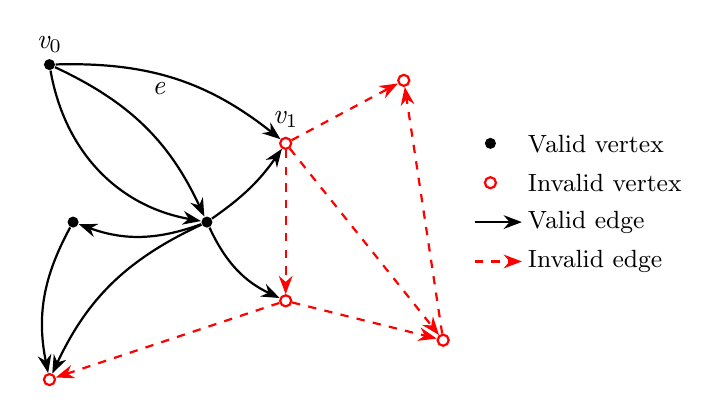
\begin{tikzpicture}
[vad/.style={circle, fill=black, inner sep=0pt, minimum size=4pt},
 inv/.style={circle, draw=red, thick, inner sep=0pt, minimum size=4pt},
 ->/.style={thick, arrows={-Stealth}}]
% \node at (0.2,0.05) {$4$}; % n1
\node[vad] (n1) at (0, 0) {};
\node at (1, 1.3) {$\m{v}_1$}; % n2
\node[inv] (n2) at (1, 1) {};
% \node at (1, -1.3) {$6$}; % n3
\node[inv] (n3) at (1, -1) {}; %
\node at (-2,2.25) {$\m{v}_0$}; % n4
\node[vad] (n4) at (-2,2) {}; 
% \node at (-2.2,-1.9) {$5$}; % n5
\node[inv] (n5) at (-2,-2) {};
% \node at (-1.7,0.2) {$3$}; % n6
\node[vad] (n6) at (-1.7,0) {};
% \node at (2.5,2.1) {$2$}; % n7
\node[inv] (n7) at (2.5,1.8) {};
% \node at (3.1,-1.3) {$7$}; % n8
\node[inv] (n8) at (3,-1.5) {};
\draw[->] (n1) to [bend right=10] (n2);
\draw[->] (n1) to [bend right=20] (n3);
\draw[->,dashed,red] (n3) to (n5);
\draw[->,dashed,red] (n3) to (n8);
\draw[->,dashed,red] (n2) to (n3);
\draw[->,dashed,red] (n2) to (n7);
\draw[->,dashed,red] (n2) to (n8);
\draw[->,dashed,red] (n8) to (n7);
\draw[->] (n4) to [bend left=20] (n1);
\draw[->] (n1) to [bend right=20] (n5);
\draw[->] (n4) to [bend left=20] (n2);
\draw[->] (n1) to [bend left=20] (n6);
\draw[->] (n6) to [bend right=20] (n5);
\draw[->] (n4) to [bend right=35] (n1);
\node at (-0.6, 1.7) {$\m{e}$};
% key on the side:
\node[vad] (n9) at (3.6, 1) {};
\node[inv] (n10) at (3.6, 0.5) {};
\draw[->] (3.4, 0) -- (4, 0);
\draw[->,dashed,red] (3.4, -0.5) -- (4, -0.5);
\node at (3.9, 1) [right=1.5pt] {\small Valid vertex};
\node at (3.9, 0.5) [right=1.5pt] {\small Invalid vertex};
\node at (3.9, 0) [right=1.5pt] {\small Valid edge};
\node at (3.9, -0.5) [right=1.5pt] {\small Invalid edge};

\end{tikzpicture}
\end{center}
\end{frame}
\colorlet{red}{stash}


\begin{frame}{Instantiating GC\_Graph}
A PreGraph is a hextuple (\texttt{VType}, \texttt{EType}, \texttt{vvalid}, \texttt{evalid}, \texttt{src}, \texttt{dst})
\begin{flushleft}
\begin{equation*}
\begin{split}
\textbf{GC\_PreGraph: } &\texttt{VType := nat * nat} \\
                    &\texttt{EType := VType * nat} \\
                    &\texttt{src := fst} \\
                    &\texttt{dst := } unrestricted \\ 
                    &\forall \m{v}.~\texttt{vvalid}(\gamma, \m{v}) \bi \texttt{graph\_has\_v}(\gamma, \m{v}) \\
                    &\forall \m{v,out}.~\texttt{evalid}(\gamma, \m{(v,out)}) \bi \\
                    &\quad \texttt{vvalid}(\gamma, \m{v}) \wedge \texttt{In } \m{out} \hspace{0.5em} (\texttt{get\_edges}(\gamma, \m{v}))
\end{split}
\end{equation*}
\end{flushleft}
\end{frame}

\begin{frame}[fragile]{Instantiating GC\_Graph}
A LabeledGraph is a quadruple (PreGraph, \texttt{VL}, \texttt{EL}, \texttt{GL})
\vspace{-1.5em}
\begin{flushleft}
\begin{equation*}
\begin{split}
\textbf{GC\_Graph: } &\text{GC\_PreGraph as shown} \\
                  &\texttt{VL := raw\_vert\_block} \\
                  &\texttt{EL := unit} \\
                  &\texttt{GL := list gen\_info} 
\end{split}
\end{equation*}
\end{flushleft}
\pause
\begin{Verbatim}
 Definition 
  raw_fld := Z + GC_Ptr.       Record gen_info :=
                               { s_addr: val;
 Record raw_vert_block :=        s_ok: isptr s_addr;
 { raw_mark: bool;               num_vert: nat;
   copied_vertex: VType;         (* elided *) }.
   raw_flds: list raw_fld;     
   (* elided *) }.             
\end{Verbatim}
\end{frame}

\begin{frame}[fragile]{\texttt{forward}: a Deep Dive}

\texttt{forward} is everywhere! 
\\\uncover<2->{\texttt{forward} is \alert{robust}}
\\\uncover<3->{\hspace{7em} pointer?} 
\uncover<4->{\hspace{1em} in \texttt{from} space?}
\uncover<5->{\hspace{1em} already forwarded?}
\\\uncover<6->{\hspace{3em}and \alert{versatile}}
\\\uncover<7->{\hspace{7em}called on root set}
\uncover<8->{\hspace{1em}called on heap}

\bigskip

\begin{Verbatim}
void forward (value *s, *l, **n, *p) { 
 value * v; value va = *p;
 if(Is_block(va)) {
  v = (value*)iop2ptr(va);
  if(Is_from(s, l, v)) {
   header_t hd = Hd_val(v);
   if(hd == 0) {
    *p = Field(v,0);
   } else { /* elided */
\end{Verbatim}
\end{frame}

\newcommand{\ga}{\gamma}
\newcommand{\tx}[1]{\text{#1}}


\begin{frame}[fragile]{\texttt{forward}: a Deep Dive}
$\braces{\forall \ga, \m{from}, \m{to}, \m{v}, \m{n}.~\p{gc{\_}graph}(\ga) \wedge \m{compat}(\ga, \m{from}, \m{to}) \wedge \null \\ \tx{s} = \m{start}(\ga, \m{from}) \wedge \tx{l} = \tx{s} + \m{gensz}(\ga, \m{from}) \wedge \null \\  \tx{n} = \m{nxtaddr}(\m{to}) \wedge \tx{p} = \m{vaddr}(\ga, \m{v}) + \m{n}} \defeq \phi_1$

\begin{Verbatim}
void forward (value *s, *l, **n, *p) { 
 /* elided */
 if(hd == 0) {
  *p = Field(v,0);
\end{Verbatim}
\pause
$\braces{\phi_{1} \wedge \exists \ga'.~\p{gc{\_}graph}(\ga') \wedge \ga' = \m{upd\_edge}(\ga, \m{e}, \m{copy}(\ga, \m{v})) \wedge \null \\ \m{compat}(\ga', \m{from}, \m{to}) \wedge \m{fwd\_relation}(\ga, \ga', \m{from}, \m{to}, \m{v}, \m{n})}$
\begin{Verbatim}
 }
\end{Verbatim}
\end{frame}

\begin{frame}[fragile]{\texttt{forward}: a Deep Dive}
\begin{Verbatim}
 else {
  int i; int sz; value *new; sz = size(hd); 
  new = *next+1; *next = new+sz; Hd_val(new) = hd;
  for(i = 0; i < sz; i++)
    Field(new, i) = Field(v, i);
\end{Verbatim}
\pause
$\braces{\phi_{1} \wedge \exists \ga', \m{v'}.~\p{gc\_graph}(\ga') \wedge 
\m{v'} = \m{copied\_vertex(\ga, \m{to})} \wedge \null \\ \ga' = \m{copy\_vertex}(\gamma, \m{to}, \m{v}, \m{v'}) \wedge \m{compat}(\ga', \m{from}, \m{to})} \defeq \phi_{2}$
\pause
\begin{Verbatim}
  Hd_val(v) = 0; Field(v, 0) = p2iop((void *)new);
  *p = p2iop((void *)new);
\end{Verbatim}
\pause
$\braces{\phi_{2} \wedge \exists \ga''.~\p{gc\_graph}(\ga'') \wedge \ga'' = \m{upd\_edge}(\ga', \m{e}, \m{v'}) \wedge \null \\ 
\m{compat}(\ga'', \m{from}, \m{to}) \wedge \m{fwd\_relation}(\ga, \ga'', \m{from}, \m{to}, \m{v}, \m{n})}$
\begin{Verbatim}
 }
\end{Verbatim}
\end{frame}

\begin{frame}[fragile]{\texttt{fwd\_relation}}
\begin{Verbatim}
Inductive fwd_relation from to : 
  forward_t -> LGraph -> LGraph -> Prop :=
\end{Verbatim}
\pause
\begin{Verbatim}
| fr_v_not_in : forall v g,
  vgen v <> from ->
  fwd_relation from to (inl (inr v)) g g
\end{Verbatim}
\pause
\begin{Verbatim}
| fr_e_to_fwded : forall e g,
  vgen (dst g e) = from ->
  raw_mark (vlabel g (dst g e)) = true ->
  let new_g := lgraph_gen_dst g e
    (copied_vertex (vlabel g (dst g e))) in
  fwd_relation from to (inr e) g new_g
\end{Verbatim}
\end{frame}

\begin{frame}[fragile]{\texttt{fwd\_relation}}
\begin{Verbatim}
| fr_e_to_not_fwded_Sn : forall e g g', 
  vgen (dst g e) = from ->
  raw_mark (vlabel g (dst g e)) = false -> 
  let new_g :=
    lgraph_gen_dst (lgraph_copy1v g (dst g e) to)
      e (copy1v_new_v g to) in 
  fwd_loop from to
    (make_fields new_g (copy1v_new_v g to)) new_g g' ->
  fwd_relation from to (inr e) g g'
\end{Verbatim} 
\end{frame}

\begin{frame}{Specification}
Similar to \texttt{forward\_relation}, we have
\\ \hspace{1em}\texttt{forward\_roots\_relation}
\\ \hspace{1em}\texttt{do\_scan\_relation}
\\ \hspace{1em}\texttt{do\_generation\_relation}
\\ \hspace{1em}\texttt{garbage\_collect\_relation}
% we specify is operationally

\bigskip

\flushright \pause A composition of these gives us our \alert{isomorphism}
\end{frame}

\begin{frame}[fragile]{Moving Towards Isomorphism}
But the journey is far from easy! 

\smallskip

A brief look at \texttt{semi\_iso}:

\bigskip

\begin{center}
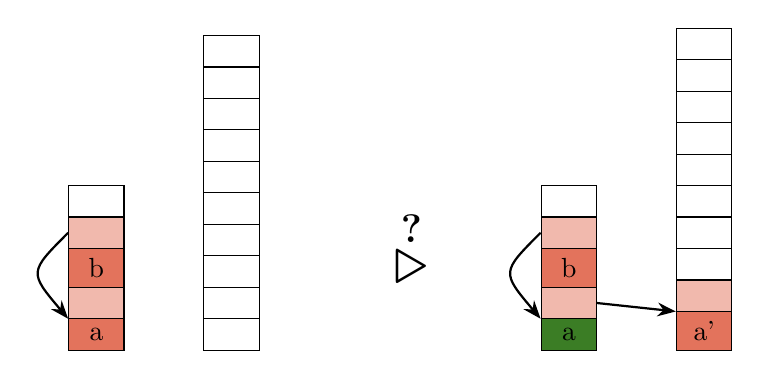
\begin{tikzpicture}[heap/.style={rectangle split, rectangle split parts=#1, draw,
        minimum width=20pt}, node distance=1cm, ->/.style={-Stealth, thick}]
\node<1-> [heap=5, rectangle split part fill={white, mypink, myred, mypink, myred}]
    (gen 0) {\nodepart{three}\ws{b}
            \nodepart{five}\ws{a}};
\node<1-> [heap=10, right = of gen 0.south east, anchor=south west,
      rectangle split part fill={white}]
        (gen 1) {};
\draw<1-> [->] (gen 0.two west)..controls ++(-0.5, -0.5).. (gen 0.four split west);

\tikzset{shift={(4,0)}}

\node<3-> {\Huge $\triangleright$};
\node<3-> at (0, 0.5) {\Large \textbf{?}};

\tikzset{shift={(2,0)}}

\node<1> [heap=5, white, rectangle split part fill={white}]
    (gen 0) {};
\node<1> [heap=10, white, right = of gen 0.south east, anchor=south west,
      rectangle split part fill={white}]
        (gen 1) {};

\node<2-> [heap=5, rectangle split part fill={white, mypink, myred, mypink, OliveGreen}]
    (gen 0) {\nodepart{three}\ws{b}
            \nodepart{five}\ws{a}};
\node<2-> [heap=10, right = of gen 0.south east, anchor=south west,
      rectangle split part fill={white, white, white, white, white, white, white, white, mypink, myred}]
        (gen 1) {\nodepart{ten}\ws{a'}};
\draw<2-> [->] (gen 0.two west)..controls ++(-0.5, -0.5).. (gen 0.four split west);
\draw<2-> [->] (gen 0.four east) -- (gen 1.nine split west);


\end{tikzpicture}
\end{center}
\end{frame}

\begin{frame}[fragile]{Moving Towards Isomorphism}

The general iterative strategy:

\bigskip

\begin{center}
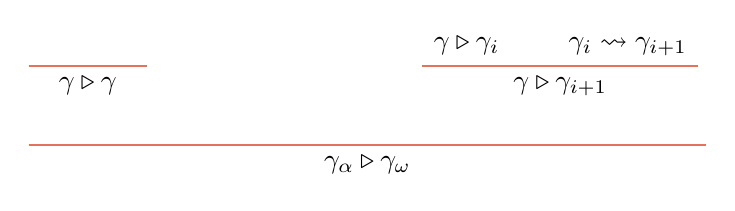
\begin{tikzpicture}
\node at (0.75,-0.25) {$\gamma \triangleright \gamma$};
\draw [thick, myred] (0,0) -- (1.5,0);
\uncover<2->{
\node at (6.75, 0.25) {$\gamma \triangleright \gamma_i \hspace{2.5em} \gamma_i \leadsto \gamma_{i+1}$};
\node at (6.75, -0.25) {$\gamma \triangleright \gamma_{i+1}$};
\draw [thick, myred] (5,0) -- (8.5,0);}
\uncover<3>{
\draw [thick, myred] (0,-1) -- (8.6,-1);
\node at (4.3,-1.25) {$\gamma_{\alpha} \triangleright \gamma_{\omega}$};}

\end{tikzpicture}
\end{center}
\end{frame}

\begin{frame}[fragile]{Moving Towards Isomorphism}

A specific example:
\begin{Verbatim}
Lemma semi_iso_refl: forall g from to,
  sound_gc_graph g -> semi_iso g g from to nil.
\end{Verbatim}
\pause
\begin{Verbatim}
Lemma fwd_rel_semi_iso:
  forall from to p g1 g2 g3 roots,
    semi_iso g1 g2 from to l1 -> 
    forward_relation from to p g2 g3 ->
    semi_iso g1 g3 from to
\end{Verbatim}
\end{frame}

\begin{frame}[fragile]{Moving Towards Isomorphism}
And eventually, 
\begin{Verbatim}
Theorem garbage_collect_iso: forall roots1 roots2 g1 g2,
  ...
  garbage_collect_relation roots1 roots2 g1 g2 ->
  gc_graph_iso g1 roots1 g2 roots2.
\end{Verbatim}

\bigskip \pause

The graphs are isomorphic
\\\hspace{1em}\alert{up to the vertices reachable from roots}\\
\pause The space between \texttt{n} and \texttt{l} is \alert{available for \texttt{alloc}}

\bigskip \pause

Note that we may still not achieve full isomorphism:
\\\pause \hspace{1em}the \alert{graph label} may change to register new vertices
\\\pause \hspace{2em}and may even grow to accommodate new generations
\end{frame}

\begin{frame}{Recap: Intuitive Specification}
\emph{Primum non nocere}: first, do no harm

\bigskip

\begin{center}
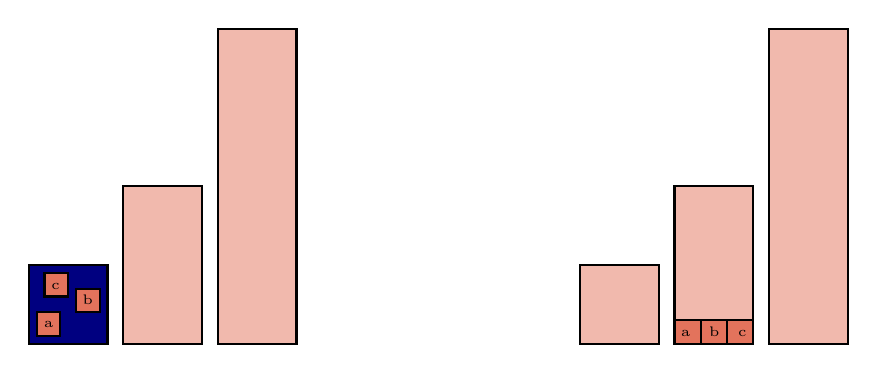
\begin{tikzpicture}
\uncover<1>{
            \draw [fill=NavyBlue, thick]
  (0,0) -- (1,0) -- (1,1) -- (0,1) -- cycle;
            \draw [fill=myred, thick]
  (0.1,0.1) -- (0.4,0.1) -- (0.4,0.4) -- (0.1,0.4) -- cycle;
            \draw [fill=myred, thick]
  (0.6,0.4) -- (0.9,0.4) -- (0.9,0.7) -- (0.6,0.7) -- cycle;
            \draw [fill=myred, thick]
  (0.2,0.6) -- (0.5,0.6) -- (0.5,0.9) -- (0.2,0.9) -- cycle;
            \draw [fill=mypink, thick ] 
  (1.2,0) -- (2.2,0) -- (2.2,2) -- (1.2,2) -- cycle;
            \draw [fill=mypink, thick ] 
  (2.4,0) -- (3.4,0) -- (3.4,4) -- (2.4,4) -- cycle;}

\node at (0.25,0.25){\tiny a};
\node at (0.75,0.56){\tiny b};
\node at (0.34,0.73){\tiny c};

\tikzset{shift={(7,0)}}
  \uncover<1>{
            \draw [fill=mypink, thick ]
  (0,0) -- (1,0) -- (1,1) -- (0,1) -- cycle;
            \draw [fill=mypink, thick ] 
  (1.2,0) -- (2.2,0) -- (2.2,2) -- (1.2,2) -- cycle;
            \draw [fill=mypink, thick ] 
  (2.4,0) -- (3.4,0) -- (3.4,4) -- (2.4,4) -- cycle;
  \draw [fill=myred, thick]
  (1.2,0) -- (2.2,0) -- (2.2,0.3) -- (1.2,0.3) -- cycle;
  \draw[thick] (1.533,0) -- (1.533,0.3);
  \draw[thick] (1.866,0) -- (1.866,0.3);
  \node at (1.7,0.15){{\tiny a} \hspace{0.01em} {\tiny b} \hspace{0.01em} {\tiny c}};}
  \end{tikzpicture}
\end{center}

\uncover<1>{\vspace{-6em}\hspace{5.8cm}\Huge $\cong$}
\end{frame}

\section{Findings}

\begin{frame}[fragile]{Bugs in the source C code}
  \begin{itemize}
  \item Cheney implemented too conservatively:\\ 
  \hspace{1em}only part of \texttt{to} space needs to be 
  \\\hspace{2em}scanned during \texttt{do\_scan}
  \pause 
  \\ Performance doubled
\pause  \bigskip
\item Overflow in the following calculation:
\begin{verbatim}
int space_size =
     h->spaces[i].limit - h->spaces[i].start;
\end{verbatim}
\pause
\hspace{1em} if difference > $2^{31}$
\pause \smallskip \\
Fixed by adjusting nursery size
  \end{itemize}
\end{frame}

\begin{frame}[fragile]{Undefined behavior in C}
 Double-bounded pointer comparisons:
    \begin{Verbatim}
int Is_from(value * lo, value * hi, value * v) {
    return (lo <= v && v < hi); }
    \end{Verbatim}
    
\begin{center}
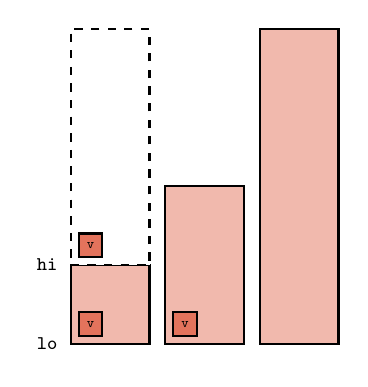
\begin{tikzpicture}
\node at (-0.3,0) {\scriptsize \texttt{lo}};
\node at (-0.3,1) {\scriptsize \texttt{hi}};

% drawing the gens
\draw [fill=mypink, thick] 
  (0,0) -- (1,0) -- (1,1) -- (0,1) -- cycle;
            \draw [fill=mypink, thick] 
  (1.2,0) -- (2.2,0) -- (2.2,2) -- (1.2,2) -- cycle;
            \draw [fill=mypink, thick] 
  (2.4,0) -- (3.4,0) -- (3.4,4) -- (2.4,4) -- cycle;

% drawing the extra malloc portion of from space
\draw<3> [fill=white, dashed, thick] 
  (0,1) -- (1,1) -- (1,4) -- (0,4) -- cycle;

% drawing v in different places
\uncover<2>{\draw [fill=myred, thick]
  (0.1,0.1) -- (0.4,0.1) -- (0.4,0.4) -- (0.1,0.4) -- cycle;
  \node at (0.25,0.25){\tiny \texttt{v}};}
\uncover<3>{\draw [fill=myred, thick]
  (0.1,1.1) -- (0.4,1.1) -- (0.4,1.4) -- (0.1,1.4) -- cycle;
  \node at (0.25,1.25){\tiny \texttt{v}};}
\uncover<4->{\draw [fill=myred, thick]
  (1.3,0.1) -- (1.6,0.1) -- (1.6,0.4) -- (1.3,0.4) -- cycle;
  \node at (1.45,0.25){\tiny \texttt{v}};}
\end{tikzpicture}
\end{center}

\uncover<5>{
Resolved using CompCert's \texttt{extcall\_properties}}
    \end{frame}

\begin{frame}[fragile]{Undefined behavior in C}  
A classic OCaml trick to disambiguate int/ptr:
    \begin{Verbatim}
int test_int_or_ptr (value x) {
    return (int)(((intnat)x)&1); }
    \end{Verbatim}

\uncover<2->{Essentially, assume that pointers are even-aligned.}
\pause \pause

\bigskip

Consider:
\begin{Verbatim}
void foo() {
  char a; char b; char* pa = &a; char* pb = &b;
  if ((pa&1 == 0) && (pb&1 == 0)) { /* elided */ } }
\end{Verbatim}

\pause
True in C, false in exec!

\bigskip

\pause Discussing \texttt{char} alignment issues with CompCert
\end{frame}



\begin{frame}{Reusability: separation between pure and spatial reasoning}
  \centering
  \includegraphics[width=0.9\textwidth]{certigc_theorems.pdf}
\end{frame}

\section{Future Work}
\begin{frame}{Future Work}
  Problems of a \alert{similar shape} \\
  \pause 
  \hspace{1em}serialization \\ 
  \hspace{1em}other collectors

  \bigskip

  \pause
  Towards a verified GC for \alert{OCaml} \\
  \pause 
  \hspace{1em}mutability \\ 
  \hspace{1em}calculate root set \\ 
  \hspace{1em}allow other datatypes

  \bigskip
  \pause \alert{Further refinements} required in C semantics \\ 
  \hspace{1em}before we can \alert{specify} and \alert{verify} OCaml's GC?
  \end{frame}


\end{document}
